\section{VGG16}

As outlined in section \ref{sec:architectures} the pre-trained VGG16 network will serve as the base-line comparison for this work. We chose VGG16 as it has a tried and true performance on labeled AT-TPC data from the $^{46}Ar$ experiment.(\cite{Kuchera2019}). For each labeled dataset listed in section \ref{sec:data} a logistic regression model was fit to the respective VGG16-representation. To estimate the variability in the result a K-fold cross validation approach was taken, with $K=5$. We report test-$f1$ scores for each class and average for the classification. The results are listed in table \ref{tab:vgg_results}

\begin{table}
\centering
\begin{tabular}{lllll}
\toprule
{} & Proton & Carbon & Other & All \\
\midrule
Simulated &  $\underset{\num{+- 1.014e-03 }  }{\num{ 0.999 } }$ &  $\underset{\num{+- 1.029e-03 }  }{\num{ 0.999 } }$ &  N/A &  $\underset{\num{+- 1.022e-03 }  }{\num{ 0.999 } }$ \\
Filtered  &  $\underset{\num{+- 5.108e-02 }  }{\num{ 0.918 } }$ &  $\underset{\num{+- 4.267e-02 }  }{\num{ 0.69 } }$ &  $\underset{\num{+- 2.359e-02 }  }{\num{ 0.908 } }$ &  $\underset{\num{+- 3.911e-02 }  }{\num{ 0.839 } }$ \\
Full      &  $\underset{\num{+- 4.653e-02 }  }{\num{ 0.84 } }$ &  $\underset{\num{+- 4.860e-02 }  }{\num{ 0.668 } }$ &  $\underset{\num{+- 1.730e-02 }  }{\num{ 0.89 } }$ &  $\underset{\num{+- 3.748e-02 }  }{\num{ 0.799 } }$ \\
\bottomrule
\end{tabular}
\caption[VGG classification results]{Logistic regression classification results using the VGG16 representation of the labeled data listed in section \ref{sec:data}. The error is given as the standard deviation in the $f1$ score over the $K=5$ folds of cross validation.}\label{tab:vgg_results}
\end{table}

 Additionally the scarceness of labeled data begs the question of how much labeled data is needed to achieve strong classification. To estimate this relationship we sample increasing subsets of the labeled data, each containing the previously selected data. For each selection a logistic regression model is fit and a $f1$ core is computed. This procedure is sensitive to which subset selected for fitting first and so a variability estimate is computed by running this procedure $N=100$ times. We report the mean and standard deviation for each dataset. The result of this analysis is shown in figure \ref{fig:vgg_n_samples}

\begin{figure}
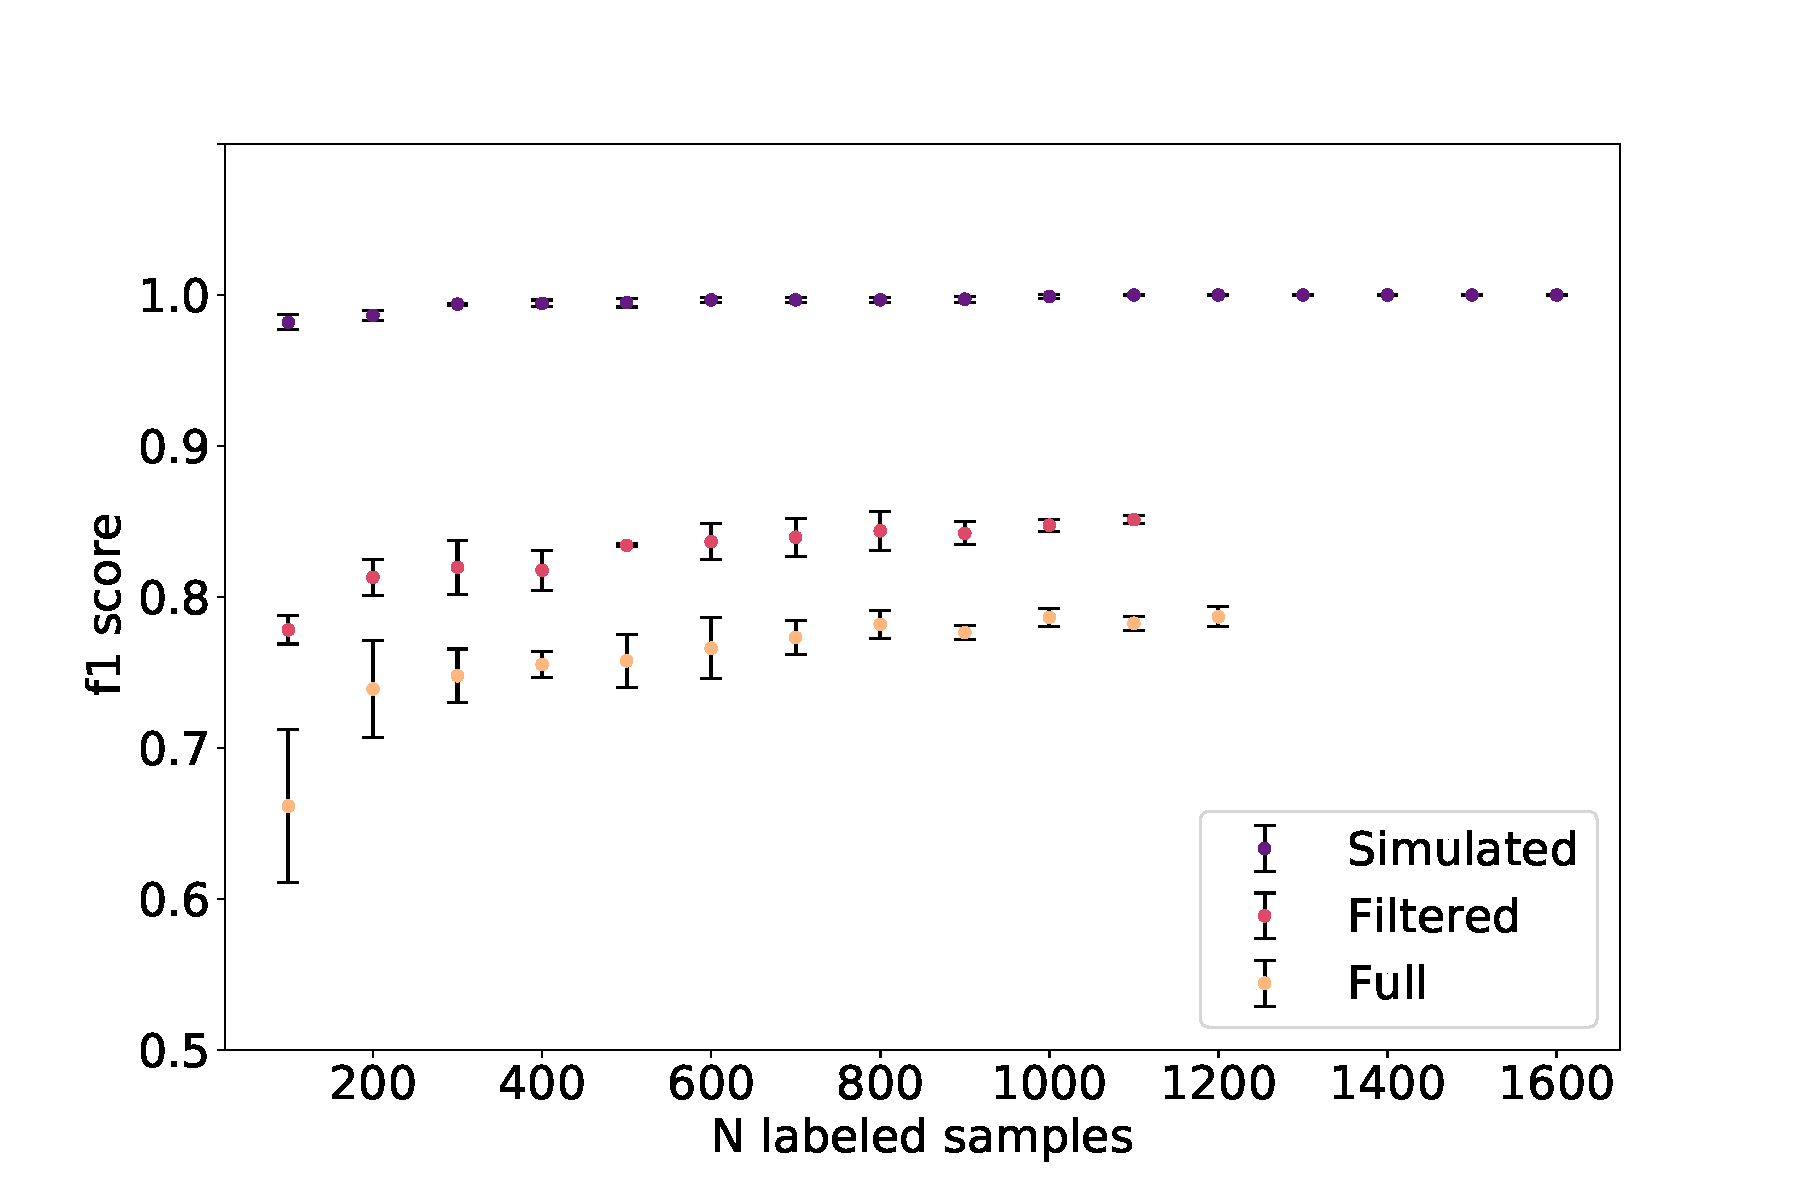
\includegraphics[width=\textwidth]{plots/vgg_n_samples.pdf}
\caption[VGG16 performance on labeled subsets]{VGG16 performance on increasing subsets of labeled data. The error-bars represent the $\pm 1\sigma$ interval from the variability in the selection of subsets. The y axis $f1$ score is computed as the unweighted average of the sample classes. }\label{fig:vgg_n_samples}
\end{figure}

For comparison we also explore a visualization of the latent space of each of the models in this thesis. The latent spaces are all however in high dimensional spaces and so we utilize a combination of a linear mapping along axes of variation (PCA) and stochastic mapping via a manifold (t-SNE). The latter renders the axes completely uninterpretable as well as making relative distances incomparable (\cite{VanDerMaaten2008}). The visualization still has some uses in that a sense of the separation of classes in the latent space can be extracted. The principal component in the t-SNE projection is the perplexity of the model essentially controlling how many neighbors the algorithms considers, recommended values lie between $perp=5$ and $perp=50$ (\cite{VanDerMaaten2008}). We chose perplexity value of $perp=15$ for all the visualizations. The latent space of the pre-trained VGG26 model is shown in figure \ref{fig:vgg_tsne} and demonstrates an evident separation of the proton class with the carbon and "other" classes. 

\begin{figure}
\centering
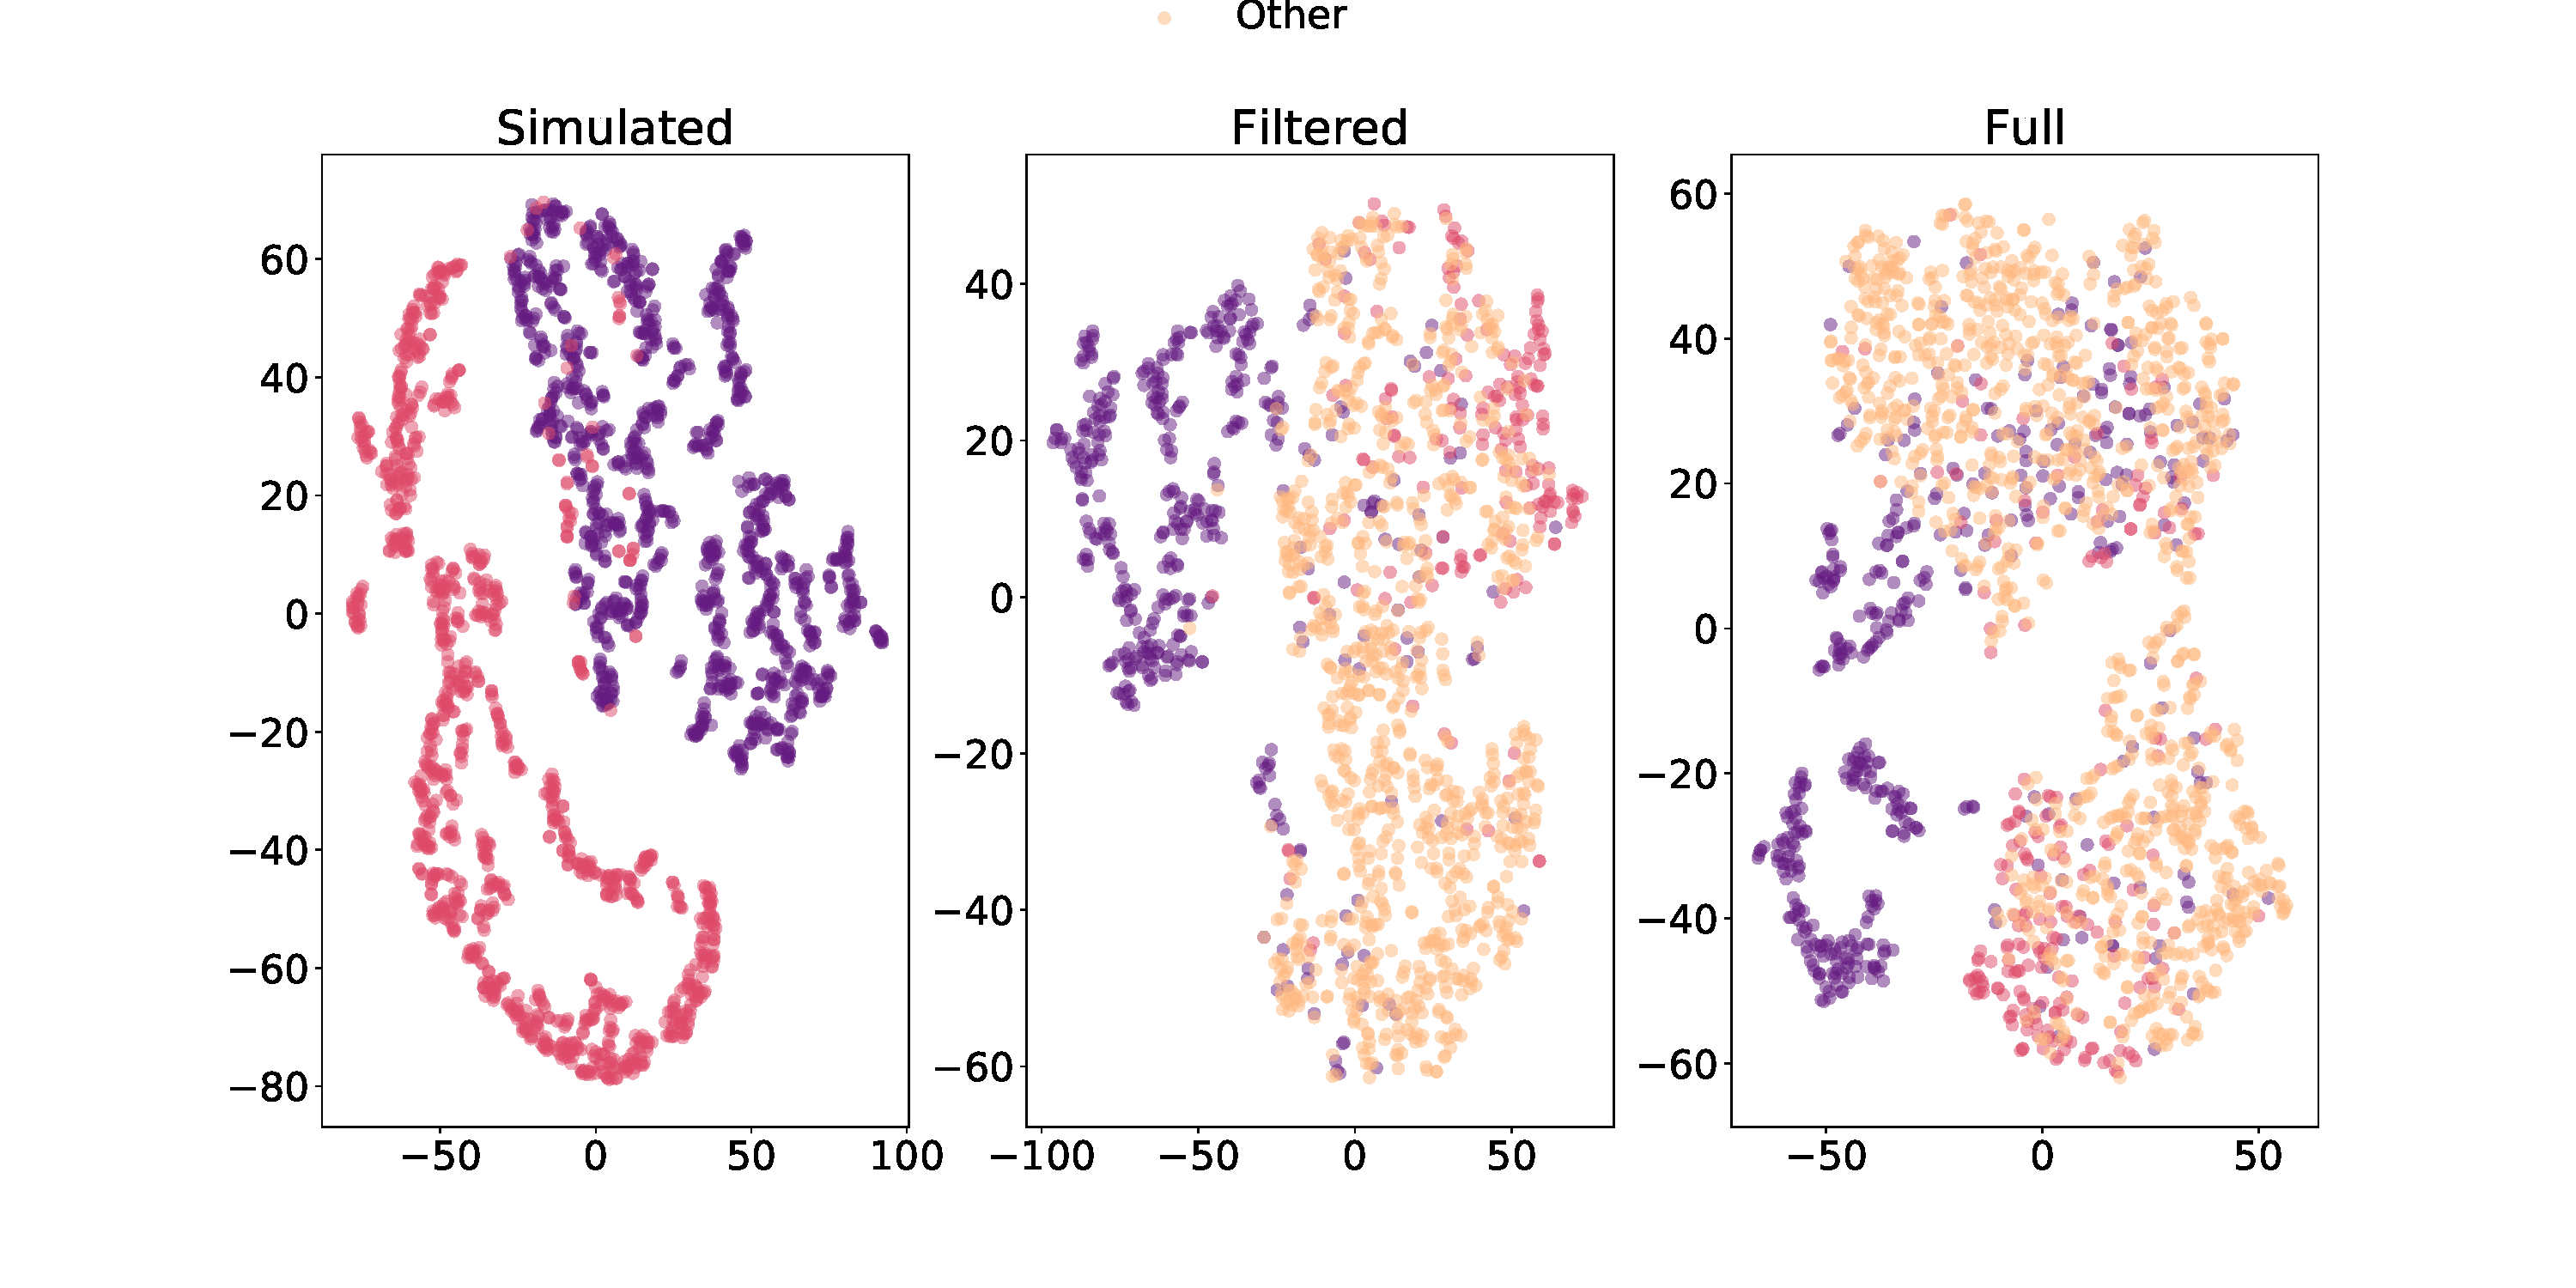
\includegraphics[width=\textwidth]{plots/vgg_tsne.pdf}
\caption[VGG16 latent visualization]{Visualization of the latent space from the VGG16 model on the three different data-sets. There is very little mixing in general between the proton class and the other two for all datasets. While the carbon and other categories seem to be mixed for the full and filtered experimental data. The axes have arbitrary non-informative units.}\label{fig:vgg_tsne}
\end{figure}